\documentclass[11pt, a4paper]{article}
% Language setting
% Replace `english' with e.g. `spanish' to change the document language

\usepackage[export]{adjustbox}

% Useful packages
\usepackage{amsmath}
\usepackage{graphicx}
\usepackage[colorlinks=true, allcolors=blue]{hyperref}
\usepackage{siunitx}
\usepackage{biblatex}
\usepackage{subcaption}



\usepackage{amsmath}
\usepackage{amsfonts} %Matheschriften
\usepackage{amssymb} %Mathesymbole
%\usepackage{mathptmx} % Einstellung für Schriften und Sonderzeichen in mathematischen Umgebungen
                        % ändert SChriftfont
\usepackage{wasysym} % Stellt diverse Sonderzeichen bereit
\usepackage{siunitx}
\usepackage{float}
\usepackage{microtype}
\usepackage{graphicx}
\usepackage{hyperref}
\usepackage{xcolor}
\usepackage[section]{placeins}
% allows for temporary adjustment of side margins
\usepackage{changepage}
\usepackage{rotating}
\usepackage{physics}

\usepackage[ngerman]{babel}

\title{Mikrofluidik Chips FoPra}
\author{Tobias Beck, Matthäus Hirsch, Benedict Brouwer}

\begin{document}
\maketitle



\section{Der Versuch}



Mikrofluidische Chips sind ein großartiger Ersatz für große und teure Laboraufbauten, da viele verschiedene Funktionen auf einem einzigen Chip implementiert werden können. In diesem Laborkurs stellen wir einen einfachen mikrofluidischen Chip her und verwenden ihn zur Messung der Diffusionskonstante von FITC in einer Agarose Lösung. 

\section{Theorie}

\subsection{Enführung}

Bei der Beobachtung von Mikrofluidik stellt man signifikante Unterschiede zu makroskopischen Flüssigkeitsströmen fest. Diese Unterschiede entstehen, da in der mikroskopischen Welt andere Effekte, wie die Elektrostatik oder auch die Grenzflächenspannung gegenüber z.B. der Gravitation dominieren. In der makroskopischen Welt ist dies genau umgekehrt. Dabei ist besonders zu beachten, dass Mikrofluidik immer laminare Strömungen aufweisen, also keine turbulenten Ströme auftreten. Zu erkennen ist dies an der sehr geringen Reynoldszahl. Durch die kleine Reynoldszahl und die laminare Strömung findet die Vermischung zweier Stoffe lediglich durch Diffusion statt und nicht wie meist sonst auch durch turbulente Strömung. Deshalb kann die Diffusionskonstante mit  Mikrofluidik Chips sehr gut bestimmt werden.
\subsection{Mathematische Beschreibung}

Die Bewegung viskoser Flüssigkeiten werden durch die Navier-Stokes Gleichungen beschrieben. Sie sind ein Set partieller Differentialgleichungen und geben als Ergebnis das Vektorfeld der Strömung an. Dabei spielen unter anderem Oberflächen Kräfte, äußere Kräfte, und die Flüssigkeit selbst eine Rolle. Aus diesen Einflussfaktoren folgt dann die Navier-Stokes Gleichung für Newtonsche Flüssigkeiten. Da diese Gleichungen oft nicht exakt gelöst werden können, sobald die Probleme komplex werden, gibt es zudem einige dimensionslose Parameter, die einfacher Auskunft über die Strömung einer Flüssigkeit geben. Damit ist die Reynoldzahl $R_{e}$ gemeint. Sie gibt an, um welche Art von Strömung es sich handelt, also laminar oder turbulent. In diesem Praktikum beschäftigen wir uns jedoch nicht so tiefgehend mit den Mathematischen Grundlagen, sondern begrenzen uns lediglich auf die Errechnung der Diffusionskonstante. 

\subsection{Mikrofluidik Chips}

Dieser Versuch betrachtet nicht allgemein Strömung und Diffusion von Flüssigkeiten, sondern speziell in einem Mikrofluidik Chip. Dieser bestehen aus miteinander verbundenen Kanälen, durch die die Flüssigkeit gezielt fließt. Durch die Kanalstruktur kann z.B. die Geschwindigkeit reguliert werden. Diese Kreisläufe können wie Strom-Kreisläufe betrachtet werden. Dann ersetzt die Flüssigkeit den Strom. Beispielsweise kann so auch der Widerstand R der Kanäle berechnet werden und ergibt sich aus den Druckunterschied $ \Delta P$ und der Flussrate Q

\begin{equation}
    R = \frac{\Delta P }{Q}.
\end{equation}

Aufgrund der sehr kleinen Kanäle handelt es sich bei Strömungen in einem Mikrofluidik Chip ausschließlich um laminare Ströme.

\subsection{Diffusion}

Für diesen Versuch spielt besonders die Diffusion eine wichtige Rolle. Sie beschreibt den Übergang zweier getrennter Stoffe zu einem homogenen Gemisch durch brownsche Molekularbewegung. Der Teilchenaustausch kann dabei durch die Formel 

\begin{equation}
    J = - D \frac{\partial c}{\partial x}
\end{equation}

beschrieben werden. Dies wird auch als Ficks erstes Gesetz bezeichnet. Dabei ist c die Konzentration eines der Stoffe, x der Weg, den ein solches Teilchen zurücklegt und D die Diffusionskonstante.  
Durch einsetzen in die Kontinuitätsgleichung und Trennung der Variablen erhält man den folgenden Ausdruck für die Errechnung der Diffusionskonstante:

\begin{equation} \label{eq:diff}
    D = \frac{< x^2 >}{ 2t }.
\end{equation}

\section{Herstellung des Chips}

Zum herstellen eines Microfluidik Chips benötigt man zuerst ein Negativ, welches die Form der Kanäle vorgibt. Dieses wird in CAD auf dem Computer designt und durch Lithographie auf einem Silizium Waver hergestellt. Bei unserem Experiment war der Siliziumwafer bereits gegeben. 
Auf dieses Negativ wurde dann flüssiges PDMS gegossen. PDMS wird dabei verwendet da es gute mechanische Eigenschaften aufweist und es sich leicht mit Glas bonden lässt. Ein weiterer Hauptgrund für die Verwendung von PDMS ist, dass es für Gase durchlässig ist, für Flüssigkeiten jedoch nicht. Dadurch kann durch den Vakuumkanal (der in Abb. 2 unterste Kanal) das restliche Gas aus den Flüssigkeitskanälen gezogen werden, sodass die Diffusionskanäle ausschließlich und vollständig mit Flüssigkeit gefüllt sind. \\

Die Produktion des Chips ist in Abbildung 1 schematisch dargestellt. Zur Herstellung des Chips wurde etwa 10g PDMS im Verhältnis 10:1 mit Härter vermischt und in eine Form aus Alufolie mit dem Siliziumnegativ gegossen. Dieses wurde durch ein Vakuum etwa 15 min entgast und anschließend eine Stunde in einem Ofen bei $80^{\circ}C$ ausgehärtet. Anschließend wurde die festgewordene Schicht PDMS vom Siliziumwafer abgelößt und das PDMS durch Abtrennen der Ränder mit einer Rasierklinge auf die Größe eines Objektträgers geschnitten. Dann wurden Ports für die Kanülen gestanzt, um Zugang zu den Kanälen unter der PDMS-Schicht zu schaffen. Abschließend wurden jedes der Mikrofluidik-Systeme mit Plasma gesäubert und auf einen Objektträger gesetzt. Dadurch entstanden die Erhebungen des Negativs als Kanäle, die unten auf dem Objektträger abschließen und nach oben durch das PDMS verschlossen sind. Der Zugang ist so nur durch die Kanülen möglich. Durch diese Kanäle können dann im folgenden Flüssigkeiten gepumpt werden um deren Verhalten auf kleinen Skalen zu untersuchen.

\begin{figure}
    \centering
    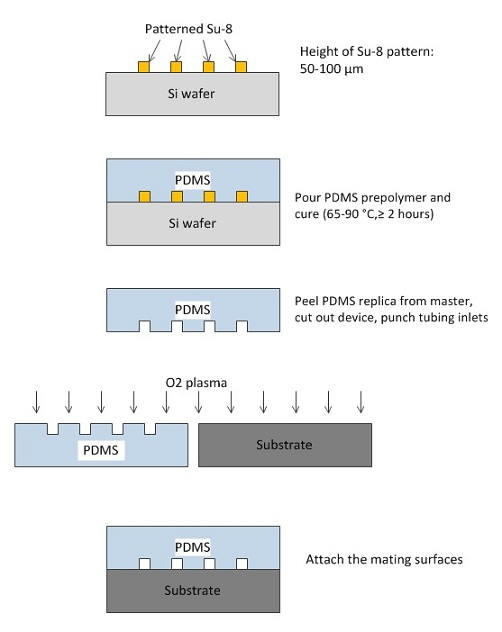
\includegraphics[width = 0.8\textwidth]{image.png}
    \caption{Herstellung und Aufbau eines PDMS Mikrofluidik Chips \cite{auf}}
    \label{fig:auf}
\end{figure}

\section{Messung der Diffusionskonstanten}

Die Messung wurde in einem optischen Mikroskop durchgeführt. Durch ein angelegtes Vakuum wurden die Seitenkanäle mit Agarose gefüllt. Anschließend wurde der Hauptkanal geflushed und mit Foureszein gefüllt. Mit dem Mikroskop wurde jede zwei Minuten sowohl im optischen als auch im FLoureszenzchannel ein Bild gemacht.

\section{Auswertung}

\begin{figure}
    \centering
    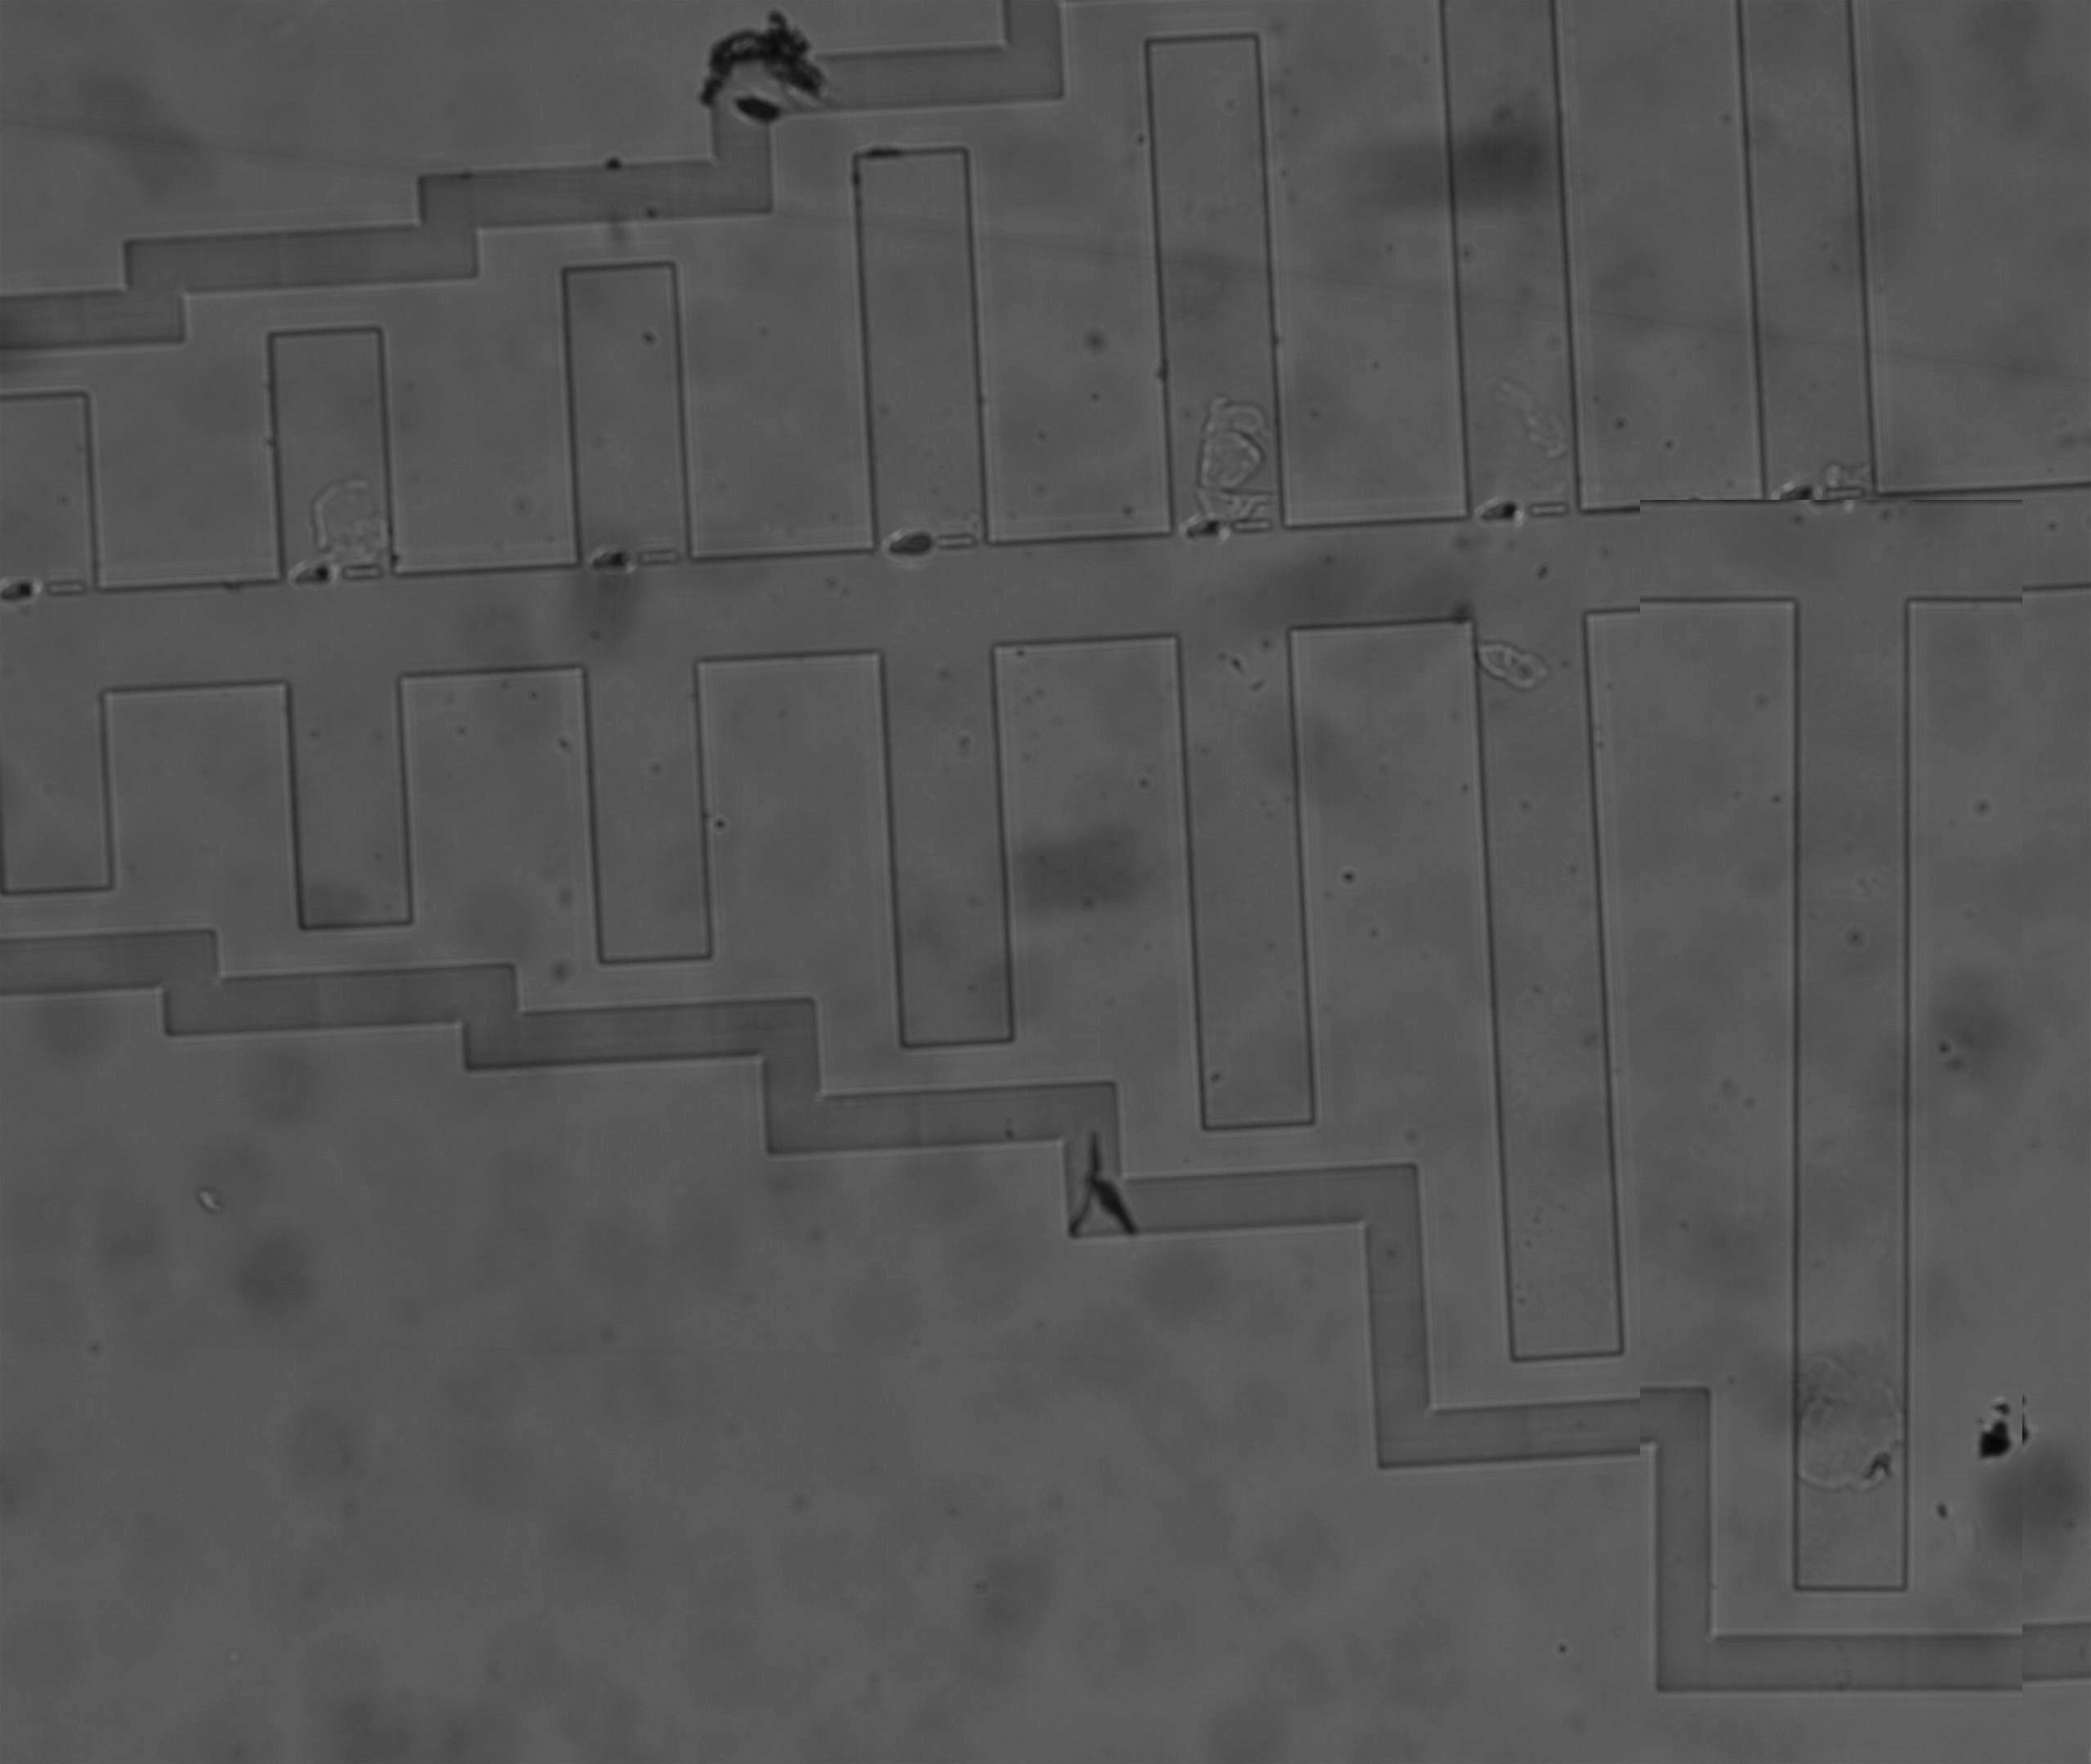
\includegraphics[scale = 0.07]{normalesFoto_heller.jpg}
    \caption{Aufnahme des Mikrofluidik Chips ohne Fluorescein}
    \label{fig:MC_boring}
\end{figure}

\begin{figure}
    \centering
    \includegraphics[scale = 0.07]{ohne erhöhten Kontrast.jpg}
    \caption{Exemplarische Aufnahme der Fluoreszenzmessung}
    \label{fig:MC_flu}
\end{figure}

\begin{figure}
    \centering
    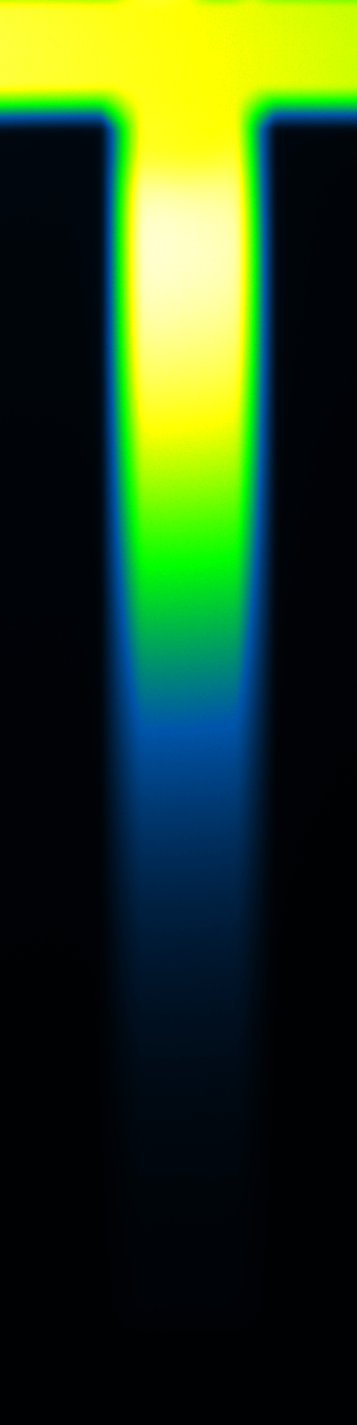
\includegraphics[scale = 0.11]{Daten_t10_c02.jpg}
    \caption{Exemplarisches Bild aus analysiertem Datensatz mit erhöhtem Kontrast}
    \label{fig:MC_contrast}
\end{figure}

\begin{figure}
    \centering
    \label{fig:MC_Analysis}
    \begin{subfigure}
    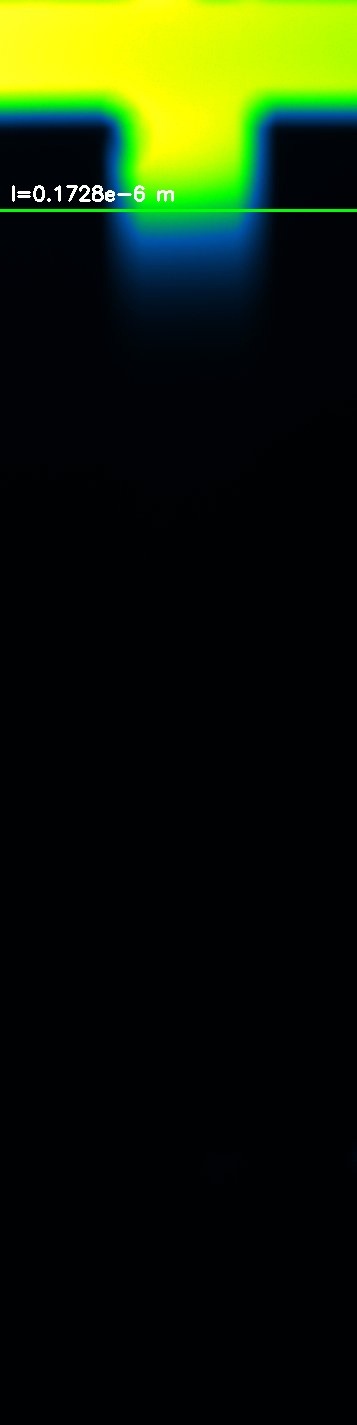
\includegraphics[width=0.11\textwidth]{Marked_Image_0.jpg}
    \end{subfigure}
    \begin{subfigure}
    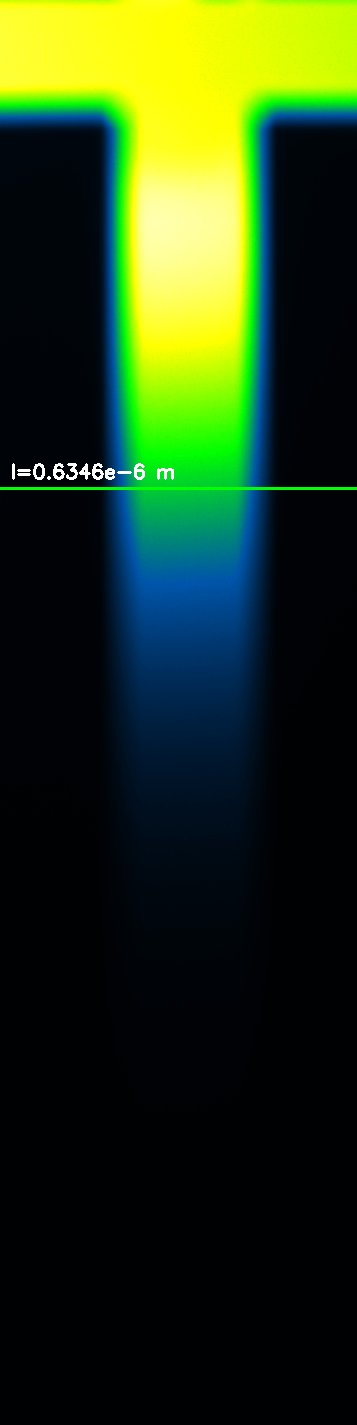
\includegraphics[width=0.11\textwidth]{Marked_Image_5.jpg}
    \end{subfigure}
    \begin{subfigure}
    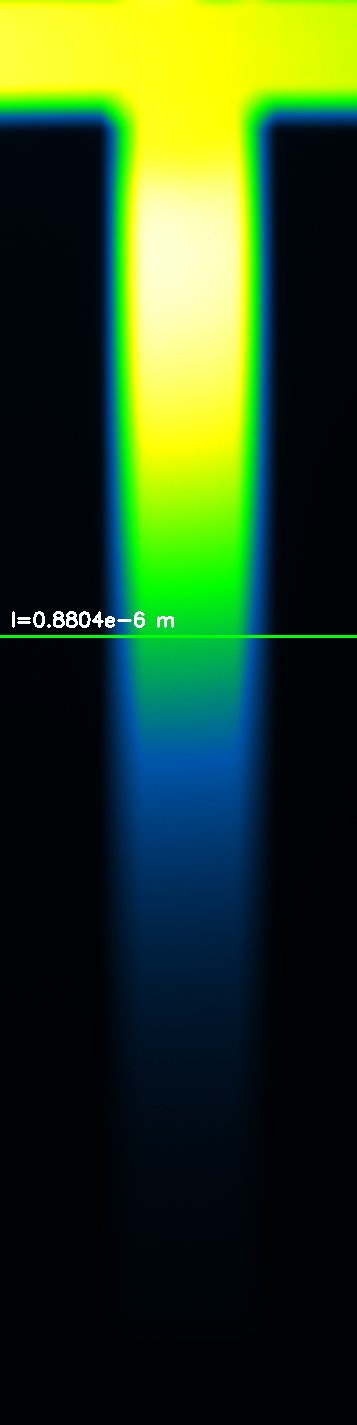
\includegraphics[width=0.11\textwidth]{Marked_Image_10.jpg}
    \end{subfigure}
    \begin{subfigure}
    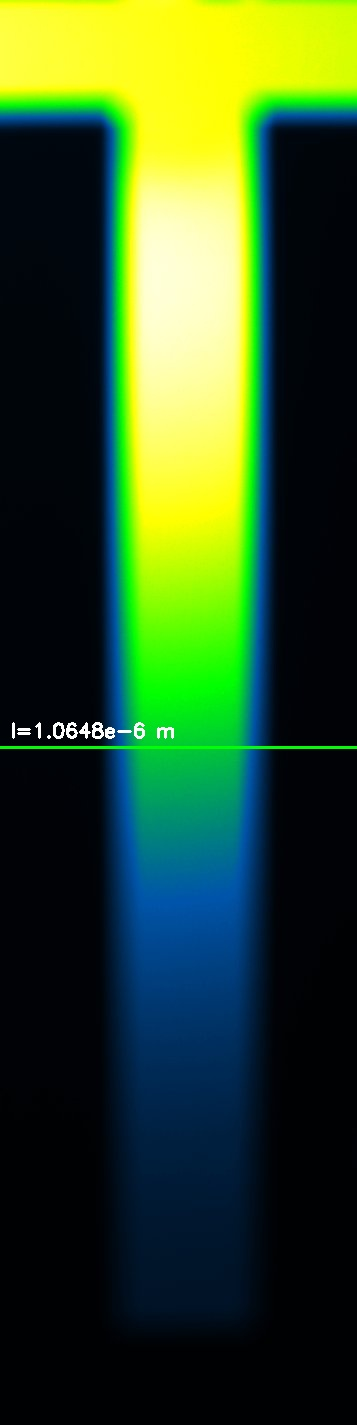
\includegraphics[width=0.11\textwidth]{Marked_Image_15.jpg}
    \end{subfigure}
    \begin{subfigure}
    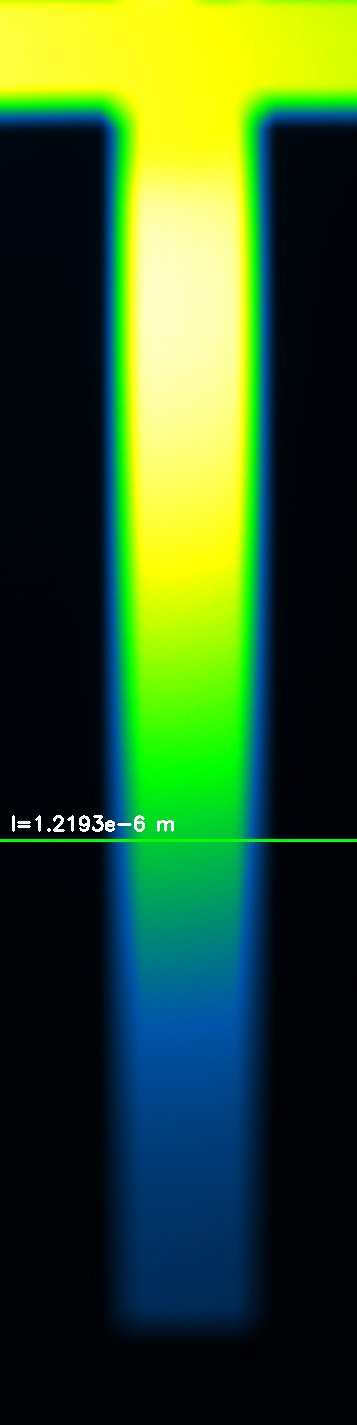
\includegraphics[width=0.11\textwidth]{Marked_Image_20.jpg}
    \end{subfigure}
    \begin{subfigure}
    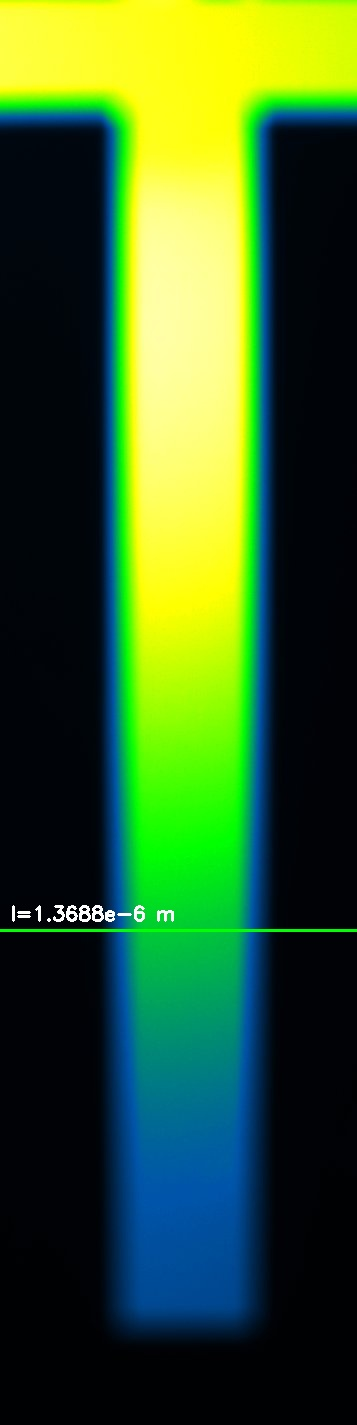
\includegraphics[width=0.11\textwidth]{Marked_Image_25.jpg}
    \end{subfigure}
    \begin{subfigure}
    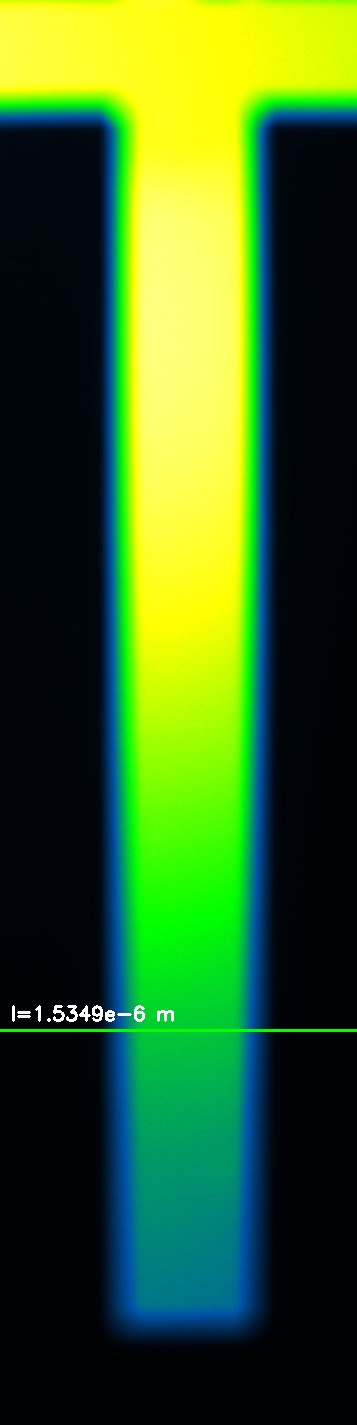
\includegraphics[width=0.11\textwidth]{Marked_Image_30.jpg}
    \end{subfigure}
    \caption{Beispiele aus der Positionsbestimmung einer bestimmten Konzentration mit gemitteltem Grünwert = 200}
\end{figure}

In Abbildungen \ref{fig:MC_boring} und \ref{fig:MC_flu} sind Mikroskopaufnahmen des verwendeten Chips zu sehen. Bild \ref{fig:MC_flu} zeigt dabei eine im Fluoreszenzkanal des Mikroskops aufgenommene Messung. Für die Auswertung wurden der letzte und längste Kanal des Chips im Fluoreszenzkanal betrachtet. Zuerst wurden die Aufnahmen mit Imagej \cite{immagejay} gedreht, zugeschnitten und die Helligkeit der Floureszenz auf ein Farbspektrum gemappt. So kann eine Veränderung der Helligkeit besser analysiert werden. In Abbildung \ref{fig:MC_contrast} ist ein derart bearbeitetes Bild dargestellt. Anschließend wurden mit einem Python Programm für die verschiedenen Zeitpunkte die Pixelpositionen einer bestimmten Grünfärbung bestimmt. Dafür wurde von unten beginnend der Grünwert über die horizontalen Pixel des Kanals gemittelt. Sobald der gemittelte Grünwert 200 überstieg wurde die Position vermerkt. Beispiele hierfür sind in Abbildung \ref{fig:MC_Analysis} zu sehen. Aus dieser Pixelposition und einer Kanallänge von $d = 2 \si{\milli\meter}$ konnte der zurückgelegte Abstand bestimmt werden. Damit kann die zu der Färbung korrespondierende Konzentration zeitlich verfolgt werden. 

\section{Ergebnis}
Die berechneten Daten wurden zusammen mit der Bildreihe und der gefitteten Diffusionsfunktion (\ref{eq:diff}) in Abbildung \ref{fig:gigaplot} dargestellt. Der Hintergrund hinter jedem Datenwert ist dabei das gemessene Fluoreszenzbild mit erhöhtem Kontrast zu diesem Zeitpunkt. Es ergibt sich durch eine Diffusionskonstante von
\begin{align}
    D = 3,1286 \pm 0,0218 \cdot 10^{-10} \si{\meter \sqared \per \second} 
\end{align}

In der Literatur konnten keine Werte für FITC mit 1\% Agarose gefunden werden, für eine 2\%ige Konzentration konnte ein Literaturwert von $ D = 0,65126 \cdot 10^{-10} \si{\meter \sqared \per \second} $ \cite{lit} bestimmt werden. Dieser ist aber erwartbarerweise viel niedriger als unser gemessener Wert, liegt aber in etwa in der gleichen Größenordnung.

\begin{figure}
    \centering
    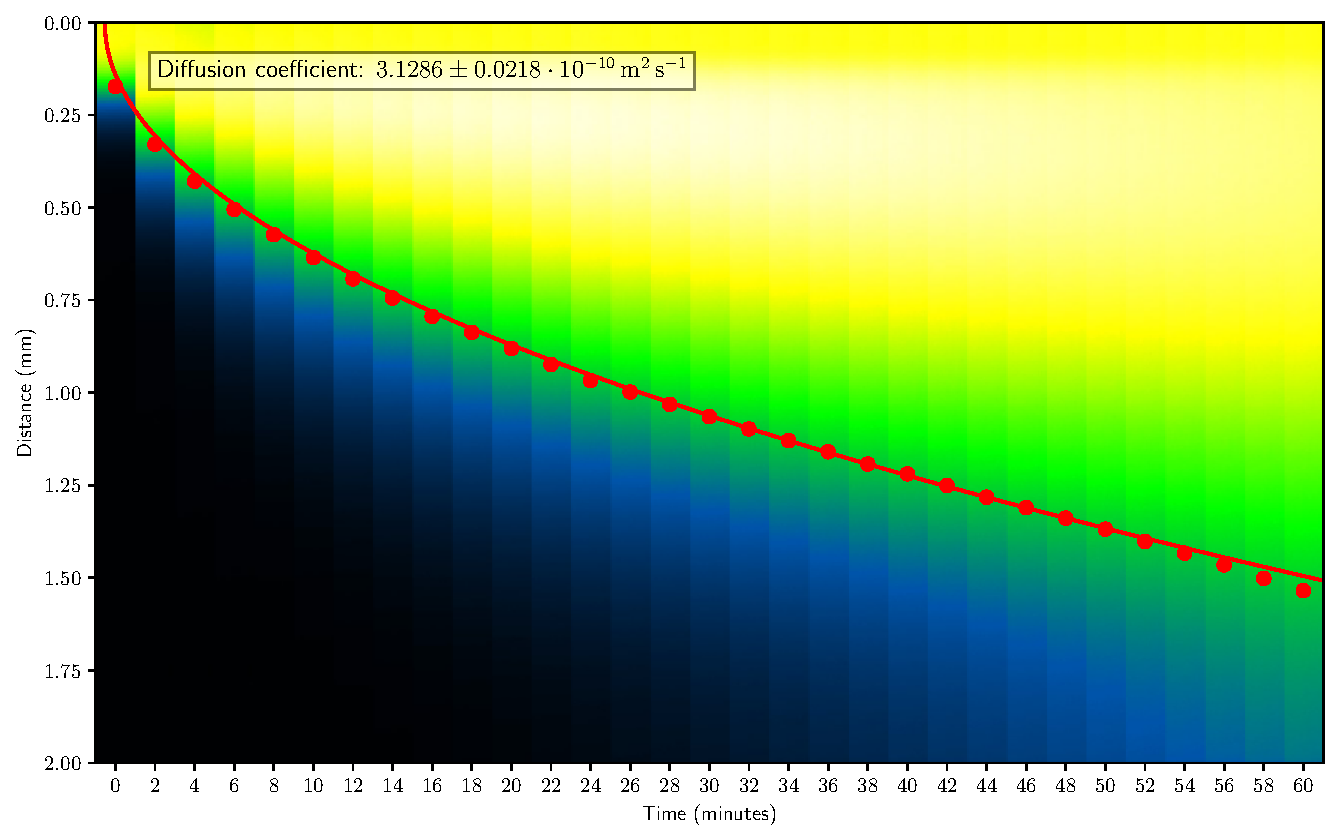
\includegraphics[max width=\linewidth]{Finalplot.pdf}
    \caption{Diffusion Abstand-Zeit-Plot mit Falschfarbenbildern}
    \label{fig:gigaplot}
\end{figure}

\bibliographystyle{alpha}
\bibliography{sample}

\end{document}

Microfluidic devices are a great substitute for big and costly lab setups, as many different functions can be implemented on a single chip. In this Lab course we manufacture a basic microfluidic chip and use it to measure the diffusion constant of agarose with a FITC solution. We determine a value of

Wir bestimmen einen Wert von $D = 3,1 \cdot 10^{10} \si{\metre\per\second}$ .